\documentclass[10pt, a5paper]{article}
\usepackage{pdfpages}
\usepackage{parallel}
\usepackage[T2A]{fontenc}
\usepackage{ucs}
\usepackage[utf8x]{inputenc}
\usepackage[polish,english,russian]{babel}
\usepackage{hyperref}
\usepackage{rotating}
\usepackage[inner=2cm,top=1.8cm,outer=2cm,bottom=2.3cm,nohead]{geometry}
\usepackage{listings}
\usepackage{graphicx}
\usepackage{wrapfig}
\usepackage{longtable}
\usepackage{indentfirst}
\usepackage{array}
\newcolumntype{P}[1]{>{\raggedright\arraybackslash}p{#1}}
\frenchspacing
\usepackage{fixltx2e} %text sub- and superscripts
\usepackage{icomma} % коскі ў матэматычным рэжыме
\PreloadUnicodePage{4}

\newcommand{\longpage}{\enlargethispage{\baselineskip}}
\newcommand{\shortpage}{\enlargethispage{-\baselineskip}}

\def\switchlang#1{\expandafter\csname switchlang#1\endcsname}
\def\switchlangbe{
\let\saverefname=\refname%
\def\refname{Літаратура}%
\def\figurename{Іл.}%
}
\def\switchlangen{
\let\saverefname=\refname%
\def\refname{References}%
\def\figurename{Fig.}%
}
\def\switchlangru{
\let\saverefname=\refname%
\let\savefigurename=\figurename%
\def\refname{Литература}%
\def\figurename{Рис.}%
}

\hyphenation{admi-ni-stra-tive}
\hyphenation{ex-pe-ri-ence}
\hyphenation{fle-xi-bi-li-ty}
\hyphenation{Py-thon}
\hyphenation{ma-the-ma-ti-cal}
\hyphenation{re-ported}
\hyphenation{imp-le-menta-tions}
\hyphenation{pro-vides}
\hyphenation{en-gi-neering}
\hyphenation{com-pa-ti-bi-li-ty}
\hyphenation{im-pos-sible}
\hyphenation{desk-top}
\hyphenation{elec-tro-nic}
\hyphenation{com-pa-ny}
\hyphenation{de-ve-lop-ment}
\hyphenation{de-ve-loping}
\hyphenation{de-ve-lop}
\hyphenation{da-ta-ba-se}
\hyphenation{plat-forms}
\hyphenation{or-ga-ni-za-tion}
\hyphenation{pro-gramming}
\hyphenation{in-stru-ments}
\hyphenation{Li-nux}
\hyphenation{sour-ce}
\hyphenation{en-vi-ron-ment}
\hyphenation{Te-le-pathy}
\hyphenation{Li-nux-ov-ka}
\hyphenation{Open-BSD}
\hyphenation{Free-BSD}
\hyphenation{men-ti-on-ed}
\hyphenation{app-li-ca-tion}

\def\progref!#1!{\texttt{#1}}
\renewcommand{\arraystretch}{2} %Іначай формулы ў матрыцы зліпаюцца з лініямі
\usepackage{array}

\def\interview #1 (#2), #3, #4, #5\par{

\section[#1, #3, #4]{#1 -- #3, #4}
\def\qname{LVEE}
\def\aname{#1}
\def\q ##1\par{{\noindent \bf \qname: ##1 }\par}
\def\a{{\noindent \bf \aname: } \def\qname{L}\def\aname{#2}}
}

\def\interview* #1 (#2), #3, #4, #5\par{

\section*{#1\\{\small\rm #3, #4. #5}}

\def\qname{LVEE}
\def\aname{#1}
\def\q ##1\par{{\noindent \bf \qname: ##1 }\par}
\def\a{{\noindent \bf \aname: } \def\qname{L}\def\aname{#2}}
}

\switchlang{ru}
\begin{document}
\title{«Клиповое мышление» и универсальный инструмент создания интерактивных учебных материалов}
\author{Сергей Чоповский, Алла Чоповская, Львов, Ukraine\footnote{\url{auslemberg@meta.ua}, \url {https://lvee.org/ru/abstracts/307}}}
\maketitle
\begin{abstract}
Do I need a struggle with students' clip thinking? In order to overcome the negative trends in the development of the “digital generation”, the teacher needs to use modern computer technolo\-gies. One of such universal tools for creating interactive educati\-onal materials is the H5P project presented here.
\end{abstract}
Каждый, кто разрабатывает и внедряет учебные электронные ресурсы, со временем сталкивается с проблемою восприятия учебного материала «поколением гаджетов». Одной из таких проблем есть «клиповое мышление» \cite{bib1} — привычка воспринимать информацию с помощью короткого, яркого, очень выразительного образа. Если ранее учащиеся без особого труда сидели на уроке 45 минут, характер обучения был в основном линейным, теперь внимание учеников можно удерживать всего лишь 15 минут. «Поколение гаджетов» больше не желает читать толстые, скучные (написанные «сухим научным языком», где «многа букаф»), с невнятными иллюстрациями учебники. Информация поступает большими хаотичными потоками, у человека не остаётся достаточно времени для глубокого и сосредоточенного её анализа. Клиповое мышление — «фильтр», защищает мозг от информационных перегрузок.  Специалисты связывают его формирование с бурным развитием информационного пространства.

Нужна ли борьба с клиповым мышлением учеников \cite{bib2}?
Умение учителя приспособить учеников к изменившимся условиям современной жизни и использовать элементы клипового мышления для организации учебного процесса, важно научить учащихся мыслить глубоко (понятийно), уметь систематизировать информацию, анализировать её, использовать для принятия обоснованных решений. Тогда «клиповость» как элемент обучения будет присутствовать, но не преобладать. Для преодоления негативных тенденций развития «цифрового поколения», учителем необходимо использование современных компьютерных технологий (без злоупотребления оными).

Одним из таких универсальных инструментов создания интерактивных учебных материалов является проект H5P \cite{bib3}. Это основанная на JavaScript среда с открытым исходным кодом, предназначенная для совместной работы, создания и совместного использования интерактивного содержимого HTML5, распространяемая под лицензией MIT \cite{bib4}.

Платформа состоит из веб-редактора контента, веб-сайта для обмена типами контента, плагинов для существующих систем управления контентом и формата файлов для объединения ресурсов \linebreak HTML5. Сам сетевой редактор умеет добавлять и заменять мультимедийные файлы, текстовое содержимое во всех видах типов контента и приложений H5P. Имеются настраиваемые виджеты для редактора, обеспечивая любые возможности редактирования всех типов контента. 

\begin{center}
\begin{figure}[h!]
  \centering
  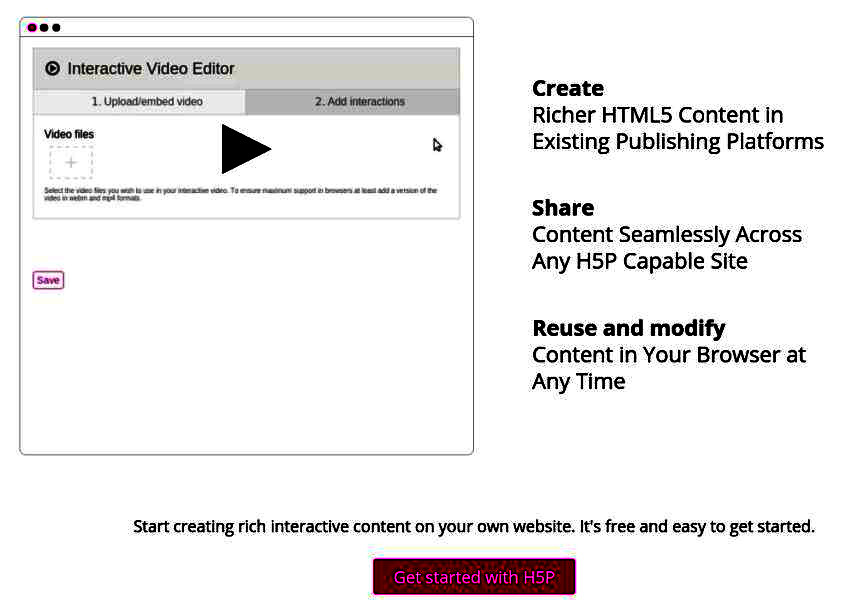
\includegraphics[width=10.8cm]{16_clip01}
  \caption{Фрагмент страницы h5p.org}
  \label{clip:fig1}
\end{figure}
\end{center}

Проект поддерживает кириллицу и снабжён хорошей справочной поддержкой. 

\begin{center}
\begin{figure}[h!]
  \centering
  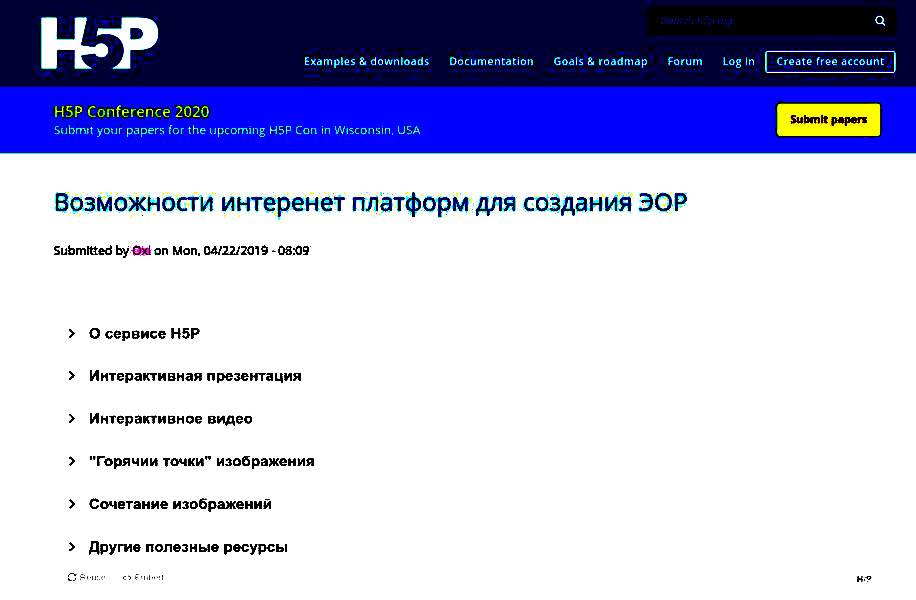
\includegraphics[width=10.8cm]{16_clip02}
  \caption{Фрагмент страницы О сервисе H5P}
  \label{clip:fig2}
\end{figure}
\end{center}

\begin{center}
\begin{figure}[h!]
  \centering
  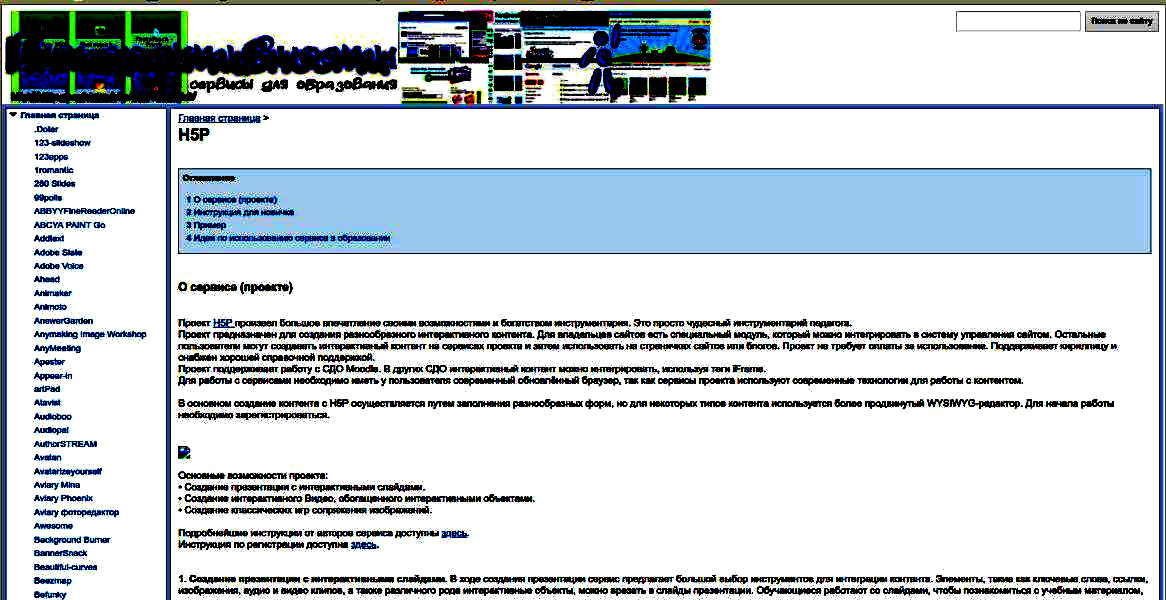
\includegraphics[width=10.8cm]{16_clip03}
  \caption{Интерактивности. Web-сервисы для образования}
  \label{clip:fig3}
\end{figure}
\end{center}

Так же проект поддерживает работу с системами ДО. Есть четыре основных плагина для Drupal, WordPress, Tiki и отдельно плагин для Moodle. В других СДО интерактивный контент можно использовать с помощью тега iFrame. Кроме выше перечисленных платформ, H5P удалось внедрить и использовать (через взаимодействие средств обучения—LTI Integration) в: Canvas (рис. \ref{clip:fig4}), Brightspace, Blackboard, LTI интеграция с Moodle, Интерактивный контент в Grav flat-file CMS,
в offline-редакторе HTML5 — \linebreak eXeLearning, добавление интерактивного контента в eXeLearning.


\begin{center}
\begin{figure}[h!]
  \centering
  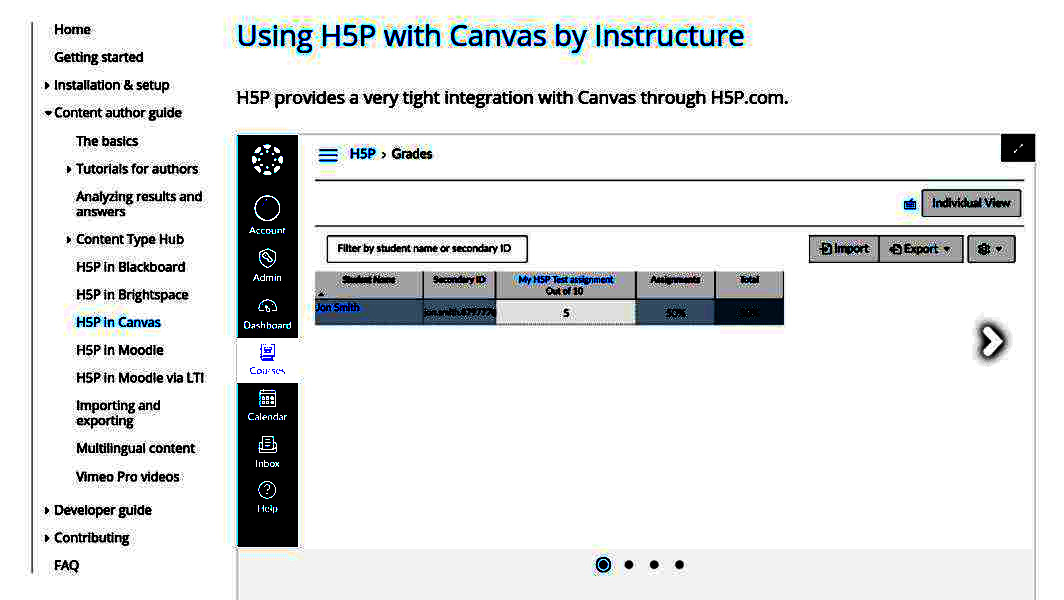
\includegraphics[width=10.8cm]{16_clip04}
  \caption{Интеграция с Canvas}
  \label{clip:fig4}
\end{figure}
\end{center} 

Кроме того H5P используется в качестве основного редактора разработки обучающего контента в diskurs LMS.
Для работы с сервисами необходимо иметь современный браузер совместимый с HTML5. Проект содержит более 40 шаблонов для создания электронных образовательных ресурсов. Основной язык проекта — английский, но большинство конструкторов в нем интуитивно понятны. И все разработки можно легко вставить на сайт или в блог. Интересно, что создание контента с H5P осуществляется путём заполнения разнообразных форм, для некоторых типов контента используется более продвинутый WYSIWYG-редактор. Рассмотрим основные возможности проекта \cite{bib5}:

\begin{itemize}
  \item Создание презентации с интерактивными слайдами: разнообразие тестовых заданий, ввод дополнительного контента, аналитические результаты тестирования, организация опроса.
  \item Создание интерактивного видео: разнообразие тестовых заданий, ввод комментариев, ввод дополнительного контента, возможность переключения к различным фрагментам видео, закладки, аналитические результаты тестирования, организация опроса.
  \item ``Горячие точки'' изображения: возможность акцентирования внимания на доступной области изображения, возможность ввода текста, изображения, видео, возможность показать изображение на большом экране.
  \item Создание классических игр сопряжения изображений: возможность увидеть объект, процесс, явление в разные периоды времени, стадии развития.
  \item Создание различных викторин: Baamboozle, Тривенты, \linebreak Myquiz.
\end{itemize}

\subsection*{Выводы}

«Клиповость»—это приобретённое качество, формируемое современными условиями существования и ритма жизни. При этом учащиеся не могут сосредоточиться, воспринимать длинные тексты, углубляться в суть, имеют крайне низкий коэффициент усвоения знаний. Неизбежность информатизации образования вызвана необходимостью использования больших объёмов информации во всех сферах деятельности и невозможностью формирования и обработки информации без помощи компьютерных технологий и средств связи.

Специалисты считают, что клиповое мышление – это не ущербность и не вина ученика, а естественный ответ на новые условия жизни. Клиповое мышление — это особенность мышления современного человека и это надо знать, чтобы помочь учащимся научиться мыслить полноценно. Для этого необходимо использовать комплексный подход, сочетая академические теоретические знания, наработку практических навыков в эксперименте и современные приёмы геймификации и мобильного обучения. Таким образом H5P (Библиотеки, приложении и типы контента) — это универсальный инструмент для создания интерактивных презентаций, видео, лент времени, плакатов, различных дидактических упражнений, опросов, игр и.т.п. Что позволяет фрагментарное представление информации увязывать с визуальными образами. При этом необходимо использовать метод дискуссий, который учит мыслить, отстаивать свою точку зрения и понимать противоположную, где поиск аргументации стимулирует логические процессы \cite{bib6}. 
Также надо использовать метод парадоксов —чтобы заставить ученика размышлять, а не просто пропускать через себя информацию. Отсутствие чётко сформулированной конечной мысли, готового вывода от учителя может заставить учащихся задуматься и задействовать логику. Приучать к чтению — научить учащихся самостоятельно выстраивать образную систему, где закрепление прочитанного (обсуждение, конспектирование и т.д.) способствует выработке умения анализировать, устанавливать связи между явлениями и, в конечном итоге, приводит к разрушению мозаичной, фрагментированной картины мира, тем самым помочь в преодолении негативных тенденций развития «цифрового поколения гаджетов».

А теперь немного фантазии: вероятно, что уже в недалёком будущем будут массово использоваться некие «обучающие машины». Скорее всего это будут «продвинутые» тренажёры (роботы) с ИИ, оснащённые аппаратурою дополненною реальностью. Их создание фактически идёт уже сейчас, и данный процесс с каждым днём все ускоряется. А вот и пример \cite{bib7}: В пресс-службе МТИ заявили, что в институте Робот-репетитор Алантим занимает должность зам.заведующего кафедрой робототехники. В будущем робот будет не только готовить учеников к экзаменам, но и проверять результаты ЕГЭ, используя искусственный интеллект. И что-то нам кажется, что и тут не обошлось без применения библиотек и приложений из H5P. Хотя несмотря на столь бурное развитие ИТ и ИИ, никакие «обучающие машины» не заменят полностью живого общения между учеником и учителем.

\begin{thebibliography}{9}
\bibitem{bib1} {{Клиповое мышление: чем отличаются «люди экрана» от «людей книги»?} \url{https://monocler.ru/klipovoe-myishlenie/}}
\bibitem{bib2} {{Клиповое мышление как фактор развития инновационных технологий в системе  образования}\url{https://znanio.ru/medianar/44/}}
\bibitem{bib3} {H5P -- Create and share rich HTML5 content and applications. \url{https://h5p.org/}}
\bibitem{bib4} {H5P is MIT Licensed. \url{https://h5p.org/MIT-licensed}}
\bibitem{bib5} {{Возможности интернет платформ для создания ЭОР}\url{https://h5p.org/node/489480}}
\bibitem{bib6} {{Клиповое мышление как проблема школьника, учителя, родителей}\url{https://en.ppt-online.org/376856}}
\bibitem{bib7} {{Робот-репетитор (МТИ) Алантим подготовит школьников к ЕГЭ}\url{https://vogazeta.ru/articles/2019/3/19/bigdata/6661-robot_repetitor_moskovskogo_tehnologicheskogo_instituta_podgotovit_shkolnikov_k_ege}}\end{thebibliography}
\end{document}
